%%%%%%%%%%%%%%%%%%%%%%%%%%%%%%%%%%%%%%%%%%%%%%%%%%%%%%%%%%%%%%%%%%%%%%%%%%%%%
%  Information Gain Prefers the Questions Users Cannot Answer
%  IEEE conference manuscript (IEEEtran, conference option)
%
%  SELF-CONTAINED: all figures are drawn inline with TikZ/pgfplots. No
%  external image files are required. Compile with pdflatex -> bibtex ->
%  pdflatex -> pdflatex.
%
%  STATUS: All sections complete. Section VII result tables and Figs. 4-5 are
%  populated from real measurements on the Music-Akenator catalogue (see
%  raig_experiment/results/*.json and the run_*.py scripts that produced
%  them). No LaTeX toolchain was available at measurement time, so this file
%  has not been compiled end-to-end (pdflatex -> bibtex -> pdflatex ->
%  pdflatex); do that before submission to catch overfull boxes / pgfplots
%  syntax issues in the newly-added Fig. 4/5 data blocks.
%%%%%%%%%%%%%%%%%%%%%%%%%%%%%%%%%%%%%%%%%%%%%%%%%%%%%%%%%%%%%%%%%%%%%%%%%%%%%

\documentclass[conference]{IEEEtran}
\IEEEoverridecommandlockouts

\usepackage{cite}
\usepackage{amsmath,amssymb,amsfonts,amsthm}
\usepackage{algorithm}
\usepackage{algpseudocode}
\usepackage{graphicx}
\usepackage{booktabs}
\usepackage{xcolor}
\usepackage{url}
\usepackage[hidelinks]{hyperref}

\usepackage{tikz}
\usepackage{pgfplots}
\usetikzlibrary{arrows.meta,positioning,shapes.geometric,calc,fit,backgrounds}
\pgfplotsset{compat=1.18}   % lower to 1.16 if your TeX distribution is older

% Binary entropy in bits, and reliability-aware information gain, evaluated
% natively by pgfmath. Fig. 3 is therefore computed, not traced.
\pgfmathdeclarefunction{Hb}{1}{%
  \pgfmathparse{-((#1)*ln(#1)+(1-(#1))*ln(1-(#1)))/ln(2)}%
}
\pgfmathdeclarefunction{RAIGf}{2}{%
  \pgfmathparse{Hb((#1)*(1-(#2))+(1-(#1))*(#2)) - Hb(#2)}%
}

\newcommand{\pend}{\textcolor{red}{\textbf{--}}}
\newcommand{\bx}{\mathbf{x}}
\newcommand{\bb}{\mathbf{b}}
\newcommand{\Hb}{H_{\mathrm{b}}}
\newcommand{\RAIG}{\mathrm{RAIG}}
\newcommand{\IG}{\mathrm{IG}}
\newcommand{\Cat}{\mathcal{C}}
\newcommand{\Qset}{\mathcal{Q}}
\newcommand{\Fset}{\mathcal{F}}

% Shared figure styles
\tikzset{
  fbox/.style   ={draw, rounded corners=1pt, align=center, inner sep=2pt,
                  minimum height=4.6mm, font=\scriptsize},
  fdata/.style  ={fbox, fill=black!5, draw=black!45},
  fproc/.style  ={fbox, fill=blue!7, draw=blue!50},
  frel/.style   ={fbox, fill=red!8,  draw=red!60, thick},
  fuser/.style  ={fbox, ellipse, fill=black!3, draw=black!55, minimum height=4mm},
  fdec/.style   ={draw, diamond, aspect=2.4, inner sep=1pt, align=center,
                  fill=black!3, font=\scriptsize},
  far/.style    ={-{Stealth[length=1.5mm]}, thin, black!70},
  frar/.style   ={-{Stealth[length=1.5mm]}, red!65, thick, densely dashed},
}

\newtheorem{proposition}{Proposition}
\newtheorem{corollary}{Corollary}
\newtheorem{definition}{Definition}

\begin{document}

\title{Information Gain Prefers the Questions Users Cannot Answer:\\
Reliability-Aware Query Selection for Interactive Identification}

\author{
\IEEEauthorblockN{Author One\IEEEauthorrefmark{1}, Author Two\IEEEauthorrefmark{1}}
\IEEEauthorblockA{\IEEEauthorrefmark{1}Department of Computer Science and Engineering\\
Institution Name, City, Country\\
Email: \{author.one, author.two\}@institution.edu}
}

\maketitle

\begin{abstract}
Interactive identification systems narrow a catalogue to a single item by
asking a sequence of binary questions, and the standard criterion for choosing
the next question is expected information gain. We show that this criterion
carries a systematic and previously unremarked defect when the answers come
from a human. Information gain rewards questions that partition the belief
evenly, but in attribute-indexed catalogues the attributes that partition most
evenly are the vague, subjective ones---mood, energy, perceived
danceability---which are precisely the attributes a user is least able to
answer correctly. The bias is aggravated by a routine preprocessing step:
binning a continuous feature at its median guarantees a maximally balanced
split, and therefore maximal apparent informativeness, for exactly the features
whose semantics are least crisp. We make three contributions. First, we
formalise interactive identification with unreliable responses as sequential
search over a per-attribute binary symmetric channel, and observe that hard
candidate elimination is the zero-noise limit of Bayesian updating rather than
a competing design; this resolves a confound that has led prior comparative
studies to attribute noise fragility to the question-selection rule when it
originates in the update rule. Second, we derive reliability-aware information
gain, the mutual information between the target and the \emph{observed}
answer, and establish that it re-ranks candidate questions rather than merely
rescaling them, that it is bounded by the per-attribute channel capacity, and
that this bound yields a query-budget lower bound of
$\log_2 N / \max_f(1-\Hb(\varepsilon_f))$. Third, we show the modification is
deployable without measuring user error rates: a three-tier annotation
distinguishing objective, semi-objective and subjective attributes is
sufficient to instantiate it. We describe a paired evaluation protocol over
homogeneous and heterogeneous noise, including the restricted-attribute
baseline that most directly threatens the method. On a 79,803-song catalogue,
per-attribute maximum information gain correlates negatively with annotated
reliability (Spearman $\rho=-0.44$, $p=0.054$ at native binning; $\rho=-0.61$,
$p=0.004$ at four bins), confirming the hypothesised bias. At the pre-registered
primary comparison (heterogeneous noise, $\lambda=1.0$), RAIG-tiered reaches
7.9\% top-1 accuracy at a fixed $T=20$ against 2.1\% for IG+soft-uniform and
0.4\% for the restricted-attribute baseline (exact McNemar $p=1.8\times10^{-9}$
and $p=2.2\times10^{-18}$ respectively), and is statistically indistinguishable
from the oracle. The advantage is noise-level dependent: RAIG-tiered trails
IG+soft-uniform at $\lambda\le0.5$ and in the noise-free control, and leads
only once the true noise is at or above the level its tiered annotation
assumes -- a limitation we report rather than obscure. A coarser two-tier
annotation recovers 82.7\% of the oracle--uniform accuracy gap.
\end{abstract}

\begin{IEEEkeywords}
interactive identification, question selection, information gain, noisy search,
Bayesian belief update, binary symmetric channel, human--computer interaction
\end{IEEEkeywords}

%=============================================================================
\section{Introduction}
%=============================================================================

\subsection{Motivation}

A recurring interaction pattern places a machine in the role of questioner and
a person in the role of oracle. A troubleshooting assistant narrows a fault by
asking about symptoms; a clinical triage tool narrows a differential by asking
about presentation; a product finder narrows a catalogue by asking about
requirements; the parlour game Akinator narrows a space of characters by asking
about traits. In each case the system holds a belief over a discrete set of
hypotheses, selects a question, observes an answer, and revises. The engineering
question is which question to ask, and the near-universal answer is the one that
maximises expected information gain.

That criterion inherits its authority from a clean theoretical setting in which
the answer is observed exactly. Human answers are not observed exactly. A user
asked whether the song they have in mind is ``energetic'' may hesitate, may
apply a personal threshold, or may simply be wrong, and the system has no way to
distinguish a considered answer from a guess. What makes this more than a
routine robustness concern is that the unreliability is not spread uniformly
over the question space. Some attributes admit near-certain answers: a listener
generally knows the performing artist and the language of the lyrics. Others
are irreducibly fuzzy, and inter-annotator agreement on affective music
descriptors is documented to be modest even among trained
annotators~\cite{hu2007mood,kim2010emotion}.

\subsection{Problem Statement}

The observation that motivates this work is that the two properties---how well
a question divides the belief, and how reliably it can be answered---are not
independent, and that their dependence appears to run in the unfavourable
direction. An attribute is vague when competent people disagree about where its
boundary falls. Disagreement distributes items on both sides of that boundary.
A near-even split is exactly what information gain rewards. The criterion
therefore has a structural tendency to promote the questions that are hardest
to answer, and it does so silently, because nothing in the objective refers to
answerability.

Standard preprocessing sharpens the effect. Continuous descriptors are
routinely discretised at the median so that they can be posed as binary
questions. A median split is a $50/50$ split by construction, which is the
maximum of the binary entropy function. The discretisation step thus assigns
peak apparent informativeness to continuous perceptual features, which are the
features users answer worst, while high-cardinality identifiers such as artist
generate only skewed, low-entropy questions and are deprioritised despite being
answerable with near certainty.

\subsection{Limitations of Existing Approaches}

Three responses to answer noise appear in the applied literature, and none
addresses the bias described above.

The first is to replace hard candidate elimination with a probabilistic belief
update, so that a contradicted candidate is downweighted rather than discarded.
This is correct and necessary, and it is where the robustness reported by
comparative studies of interactive identification actually originates. It does
not change which questions are asked.

The second is to learn a question-selection policy from simulated interaction,
typically by regressing the realised reduction in candidate-set size onto
features of the state and the query. This substitutes an approximation for a
quantity that has a closed form under the model, and in the absence of an
explicit noise term the learned policy inherits the same bias from its training
signal.

The third is to discard unreliable attributes altogether. This is a reasonable
practitioner heuristic and we treat it as a baseline, but it is wasteful: an
attribute answered correctly seventy per cent of the time still transmits
information, and discarding it removes that information permanently rather than
deferring its use to the point where more reliable questions have been
exhausted.

\subsection{Research Gap}

The theory needed to correct the bias is not new. Noisy search has been studied
since R\'enyi~\cite{renyi1961} and Ulam~\cite{ulam1976}, surveyed
comprehensively by Pelc~\cite{pelc2002}, and placed on a decision-theoretic
footing by Jedynak et al.~\cite{jedynak2012}, who show that greedily minimising
expected posterior entropy is optimal over the full horizon under a stated
observation model. Bayesian experimental design supplies the general
principle~\cite{lindley1956,chaloner1995}. What is missing is the empirical
observation that in attribute-indexed catalogues the observation model is
strongly heterogeneous across attributes and adversarially aligned with the
naive acquisition function, together with a deployable account of what a
practitioner must actually know to correct it. The literature on noisy twenty
questions typically assumes a single known crossover probability; the applied
literature typically assumes none at all.

\subsection{Contributions}

\begin{enumerate}
\item \textbf{A characterisation of the bias.} We formalise the relationship
between per-attribute information gain and per-attribute answerability and
provide a protocol for measuring it in any attribute-indexed catalogue,
including the contribution of the discretisation step itself
(Section~\ref{sec:setup}).

\item \textbf{A unification that removes a standing confound.} Hard elimination
is the $\varepsilon \to 0$ limit of the Bayesian update
(Proposition~\ref{prop:limit}). Comparative studies that pair an
information-gain selector with elimination and a learned selector with soft
updating vary two factors simultaneously; their conclusions about selection
strategy do not follow. We separate the factors explicitly
(Section~\ref{sec:baselines}).

\item \textbf{Reliability-aware information gain.} We derive the acquisition
function $\RAIG(q) = \Hb(p_q \star \varepsilon_q) - \Hb(\varepsilon_q)$, show
that it re-ranks rather than rescales (Proposition~\ref{prop:reversal}), and
derive a capacity-based lower bound on the query budget
(Corollary~\ref{cor:budget}). The change is one line in an existing selector.

\item \textbf{A deployability result.} We show how to instantiate the method
from a three-tier qualitative annotation rather than measured error rates, and
design the experiment to quantify how much of the oracle benefit survives that
coarsening (Section~\ref{sec:ablation}).

\item \textbf{An open reference implementation and evaluation harness} with
paired sampling, exact McNemar testing, and the restricted-attribute baseline
that most threatens the method.
\end{enumerate}

%=============================================================================
\section{Background and Related Work}
%=============================================================================

\subsection{Searching with Errors}

The problem of identifying an unknown element through queries whose answers may
be wrong originates with R\'enyi's formulation of a guessing game in which the
responder lies with fixed probability~\cite{renyi1961}, and independently with
Ulam's question of how many yes/no queries suffice to locate an integer below
one million when a bounded number of answers may be false~\cite{ulam1976}. The
combinatorial branch, in which lies are adversarial and bounded in number,
produces optimal strategies with a direct correspondence to error-correcting
codes; Pelc's survey remains the standard reference~\cite{pelc2002}. The
probabilistic branch treats errors as channel noise and connects to sequential
transmission with feedback~\cite{horstein1963,burnashev1974}, to noisy binary
search~\cite{karp2007,nowak2011}, and to modern treatments in which the noise
depends on the query itself~\cite{kaspi2018,chung2018}.

Our setting sits in the probabilistic branch, with one departure that turns out
to matter. Existing formulations assume a single crossover probability, or make
it depend on a continuous query parameter. In an attribute catalogue the
crossover is a property of the semantic category being probed and varies by an
order of magnitude across categories. That heterogeneity, rather than the
presence of noise as such, is what drives the effect we report.

\subsection{Information-Theoretic Query Selection}

Choosing the experiment that maximises expected information about a latent
quantity is the central prescription of Bayesian experimental
design~\cite{lindley1956,chaloner1995}, and in the noiseless binary case it
reduces to maximising the entropy of the induced partition. Jedynak et
al.~\cite{jedynak2012} give the result most relevant here: for twenty questions
with noise under entropy loss, a greedy one-step policy is optimal over the
whole horizon. We rely on that result rather than compete with it. Our claim is
not that greedy entropy minimisation is the wrong policy but that it is
routinely applied with the noise term omitted, and that the omission is not
benign when the noise is heterogeneous.

\subsection{Interactive and Conversational Recommendation}

Systems that alternate between asking about attributes and proposing items form
a substantial literature, including policy-learning approaches over
knowledge graphs~\cite{lei2020ear,lei2020cpr,deng2021unicorn}. Maximum-entropy
attribute querying appears throughout as a standard baseline against which
learned policies are compared. This positions our work carefully: we are not
proposing a competitor to learned conversational policies but a correction to
the baseline those policies are measured against, which is a modest claim and
we make no larger one. The correction is orthogonal and could be applied inside
a learned policy's action-scoring step.

\subsection{Question Asking in Language Models}

Recent work evaluates and improves the information-seeking behaviour of
language models, using twenty-questions style tasks as the
testbed~\cite{debruyn2022,mazzaccara2024,hu2024uot}. These systems generate
questions in open natural language rather than selecting from a fixed
attribute-value grid, which makes them more flexible and considerably more
expensive per turn. The bias we describe should apply to them as well, since
expected-information-gain reranking of generated
questions~\cite{mazzaccara2024} inherits the same blind spot, but verifying
that is beyond the present scope and we flag it as future work rather than
claiming it.

\subsection{Positioning}

Table~\ref{tab:related} places this work against the closest prior art. The
honest summary is that the acquisition function we derive is standard mutual
information under a stated observation model, and its derivation is
unsurprising to anyone working in Bayesian experimental design. The
contribution we claim is empirical and diagnostic: that the observation model
in attribute catalogues is heterogeneous in a specific and unfavourable way,
that this is partly an artefact of preprocessing rather than of the domain, and
that correcting it requires less knowledge than one might expect.

\begin{table}[t]
\caption{Positioning against closest prior work.}
\label{tab:related}
\centering
\footnotesize
\begin{tabular}{@{}lccc@{}}
\toprule
\textbf{Work} & \textbf{Noise} & \textbf{Heterog.\ $\varepsilon$} & \textbf{Selection} \\
\midrule
R\'enyi~\cite{renyi1961}, Ulam~\cite{ulam1976} & yes & no & theory \\
Pelc~\cite{pelc2002} (survey) & yes & no & optimal \\
Jedynak et al.~\cite{jedynak2012} & yes & no & greedy entropy \\
Karp \& Kleinberg~\cite{karp2007} & yes & no & noisy bisection \\
Kaspi et al.~\cite{kaspi2018} & yes & query-dep. & information-theoretic \\
EAR / CPR / UNICORN~\cite{lei2020ear,lei2020cpr,deng2021unicorn} & no & no & learned policy \\
Max-entropy baseline & no & no & classical IG \\
UoT~\cite{hu2024uot}, \cite{mazzaccara2024} & implicit & no & EIG over text \\
\midrule
\textbf{This work} & yes & \textbf{per-attribute} & \textbf{RAIG} \\
\bottomrule
\end{tabular}
\end{table}

%=============================================================================
\section{System Design}
%=============================================================================

\subsection{Overall Architecture}

The system is organised as five components arranged around a single mutable
object, the belief vector. Fig.~\ref{fig:arch} shows the arrangement. A
\emph{catalogue compiler} converts a table of items and categorical attributes
into a boolean question matrix, materialising once what would otherwise be
recomputed at every turn. A \emph{reliability model} supplies a crossover
probability for each attribute. A \emph{query selector} scores every unasked
question against the current belief and the reliability vector and returns an
argmax. An \emph{inference engine} applies Bayes' rule to the observed answer.
A \emph{termination controller} decides between asking again and committing to
a prediction.

%---------------------------------------------------------------- Fig. 1
\begin{figure}[t]
\centering
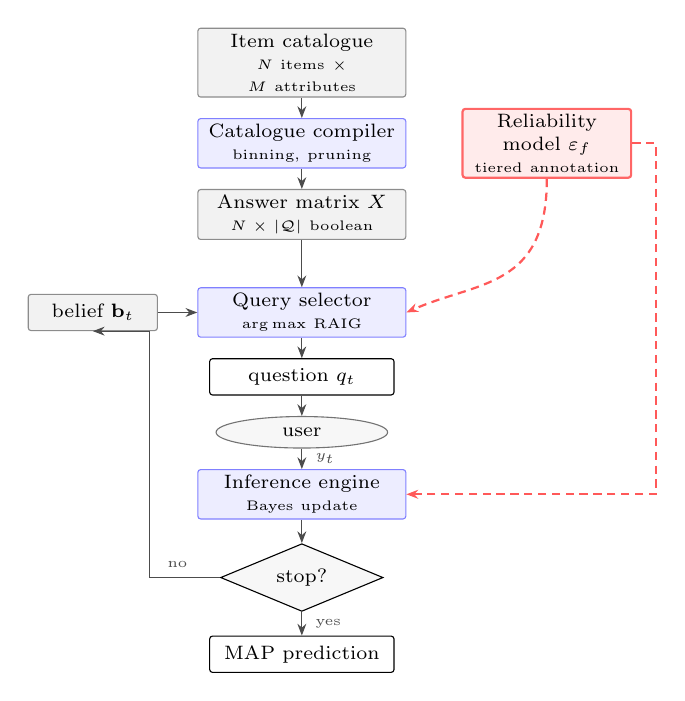
\begin{tikzpicture}[node distance=2.6mm]

\node[fdata, text width=25mm] (cat) {Item catalogue\\{\tiny $N$ items $\times$ $M$ attributes}};
\node[fproc, text width=25mm, below=of cat] (comp)
  {Catalogue compiler\\{\tiny binning, pruning}};
\node[fdata, text width=25mm, below=of comp] (X)
  {Answer matrix $X$\\{\tiny $N\times|\Qset|$ boolean}};

\node[frel, text width=20mm, right=7mm of comp] (rel)
  {Reliability\\model $\varepsilon_f$\\{\tiny tiered annotation}};

\node[fproc, text width=25mm, below=6mm of X] (sel)
  {Query selector\\{\tiny $\arg\max$ RAIG}};
\node[fdata, text width=15mm, left=5mm of sel] (bel) {belief $\bb_t$};

\node[fbox, text width=22mm, below=of sel] (q) {question $q_t$};
\node[fuser, text width=14mm, below=of q] (user) {user};
\node[fproc, text width=25mm, below=of user] (inf)
  {Inference engine\\{\tiny Bayes update}};
\node[fdec, text width=13mm, below=3mm of inf] (term) {stop?};
\node[fbox, text width=22mm, below=3mm of term] (out) {MAP prediction};

\draw[far] (cat) -- (comp);
\draw[far] (comp) -- (X);
\draw[far] (X) -- (sel);
\draw[far] (bel) -- (sel);
\draw[far] (sel) -- (q);
\draw[far] (q) -- (user);
\draw[far] (user) -- node[right, font=\tiny, xshift=0.5mm] {$y_t$} (inf);
\draw[far] (inf) -- (term);
\draw[far] (term) -- node[right, font=\tiny, xshift=0.5mm] {yes} (out);

% belief feedback loop
\draw[far] (term.west) -- ++(-9mm,0) node[above, font=\tiny, pos=0.6] {no}
           |- (bel.south);

% the two reliability arrows -- the point of the figure
\draw[frar] (rel.south) .. controls +(0,-14mm) and +(9mm,4mm) .. (sel.east);
\draw[frar] (rel.east) -- ++(3mm,0) |- (inf.east);

\end{tikzpicture}
\caption{System architecture. The reliability model is consumed by both the
selector and the inference engine (dashed); existing systems typically consume
it in the latter only, which is the omission this work addresses.}
\label{fig:arch}
\end{figure}
%----------------------------------------------------------------------

The design decision worth stating explicitly is that the reliability model is
consumed in two places rather than one. Systems that model answer noise at all
generally do so in the likelihood, where it prevents a wrong answer from
destroying the posterior. Feeding the same quantity into the selector is what
prevents the wrong answer from being solicited in the first place.

\subsection{Component Design}

Table~\ref{tab:modules} lists the modules and their responsibilities. Each
selector is a pure function of belief, question matrix and reliability vector,
with no internal state; sessions are driven entirely by an externally supplied
random stream. This is not incidental tidiness. It is what allows the same
target and the same noise realisation to be replayed across every method under
comparison, which in turn is what licenses paired statistical testing.

\begin{table}[t]
\caption{Module responsibilities.}
\label{tab:modules}
\centering
\footnotesize
\begin{tabular}{@{}p{0.24\columnwidth}p{0.66\columnwidth}@{}}
\toprule
\textbf{Module} & \textbf{Responsibility} \\
\midrule
\texttt{compile\_catalogue} & Materialise the $N \times |\Qset|$ boolean answer matrix; drop degenerate questions \\
\texttt{discretize} & Quantile-bin continuous attributes; record which were binned \\
\texttt{tiered\_reliability} & Map qualitative attribute tiers to $\varepsilon$ \\
\texttt{select\_*} & Query selectors (random, IG, RAIG, restricted IG) \\
\texttt{soft\_update} / \texttt{hard\_update} & Posterior revision under BSC$(\varepsilon)$ and its $\varepsilon\!\to\!0$ limit \\
\texttt{run\_session} & One identification episode under a fixed budget \\
\texttt{run\_paired\_experiment} & Common-random-number evaluation across methods \\
\texttt{mcnemar}, \texttt{paired\_bootstrap\_ci} & Paired inference \\
\texttt{measure\_pathology} & Per-attribute IG against reliability \\
\bottomrule
\end{tabular}
\end{table}

\subsection{Data Flow}

Fig.~\ref{fig:dataflow} traces one turn. The belief vector and the question
matrix meet in a single matrix--vector product that yields the split mass of
every candidate question at once; the reliability vector transforms those split
masses into scores; the argmax is posed; the observed answer and the same
reliability vector produce a likelihood; the posterior is renormalised. The
loop carries no state other than the belief and the set of asked questions.

%---------------------------------------------------------------- Fig. 2
\begin{figure}[t]
\centering
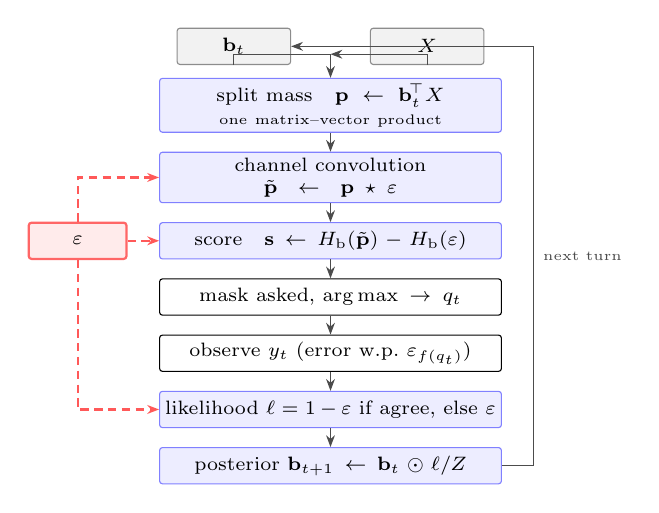
\begin{tikzpicture}[node distance=2.4mm]

\node[fdata, text width=13mm] (b) {$\bb_t$};
\node[fdata, text width=13mm, right=10mm of b] (X) {$X$};

\node[fproc, text width=42mm, below=4mm of $(b)!0.5!(X)$] (mv)
  {split mass\quad $\mathbf{p} \gets \bb_t^{\!\top}X$\\{\tiny one matrix--vector product}};
\node[fproc, text width=42mm, below=of mv] (conv)
  {channel convolution\\$\tilde{\mathbf{p}} \gets \mathbf{p}\star\varepsilon$};
\node[fproc, text width=42mm, below=of conv] (sc)
  {score\quad $\mathbf{s} \gets \Hb(\tilde{\mathbf{p}}) - \Hb(\varepsilon)$};
\node[fbox, text width=42mm, below=of sc] (am)
  {mask asked, $\arg\max \rightarrow q_t$};
\node[fbox, text width=42mm, below=of am] (y)
  {observe $y_t$ (error w.p.\ $\varepsilon_{f(q_t)}$)};
\node[fproc, text width=42mm, below=of y] (lik)
  {likelihood $\ell = 1-\varepsilon$ if agree, else $\varepsilon$};
\node[fproc, text width=42mm, below=of lik] (post)
  {posterior $\bb_{t+1} \gets \bb_t \odot \ell / Z$};

\node[frel, text width=11mm, left=4mm of sc] (eps) {$\varepsilon$};

\draw[far] (b) |- ([yshift=3mm]mv.north) -- (mv.north);
\draw[far] (X) |- ([yshift=3mm]mv.north);
\draw[far] (mv) -- (conv);
\draw[far] (conv) -- (sc);
\draw[far] (sc) -- (am);
\draw[far] (am) -- (y);
\draw[far] (y) -- (lik);
\draw[far] (lik) -- (post);

\draw[frar] (eps.north) |- (conv.west);
\draw[frar] (eps.east) -- (sc.west);
\draw[frar] (eps.south) |- (lik.west);

\draw[far] (post.east) -- ++(4mm,0) |- node[right, font=\tiny, pos=0.25] {next turn} (b.east);

\end{tikzpicture}
\caption{Data flow for a single turn. The reliability vector $\varepsilon$
enters three times: twice on the selection path and once on the inference path.}
\label{fig:dataflow}
\end{figure}
%----------------------------------------------------------------------

\subsection{Design Rationale}

Three choices deserve justification. Materialising the answer matrix trades
$O(N|\Qset|)$ bits of memory for the elimination of all per-turn recomputation,
reducing selection to one matrix--vector product and a vectorised transform;
for catalogues of the size considered here the memory is negligible and the
saving is what makes exhaustive scoring of the question space tractable.
Keeping selectors stateless costs a small amount of parameter passing and buys
the paired experimental design. Representing reliability per attribute rather
than per question reflects the belief that answerability is a property of the
semantic category rather than of the particular value being probed; a user who
is unsure whether a song is energetic is unsure regardless of the threshold,
whereas per-question estimation would multiply the annotation burden by the
number of distinct values.

%=============================================================================
\section{Methodology}
\label{sec:method}
%=============================================================================

\subsection{Notation and Problem Formulation}

Let $\Cat = \{c_1,\dots,c_N\}$ be a catalogue and
$\Fset = \{f_1,\dots,f_M\}$ a set of categorical attributes, with $a_f(c)$
denoting the value of attribute $f$ for item $c$. A question is a pair
$q=(f,v)$ with answer function
\begin{equation}
x_q(c) \;=\; \mathbb{1}\!\left[a_f(c)=v\right] \in \{0,1\},
\end{equation}
and $\Qset$ collects all non-degenerate questions. Write $\bx_q \in \{0,1\}^N$
for the column vector of answers and $f(q)$ for the attribute probed by $q$.

The system maintains a belief $\bb_t \in \Delta^{N-1}$, initialised uniform. At
each step it selects $q_t \in \Qset$, observes $y_t \in \{0,1\}$, and updates.
A session runs for at most $T$ questions and terminates with the maximum a
posteriori item. Table~\ref{tab:notation} collects the notation.

\begin{table}[t]
\caption{Notation.}
\label{tab:notation}
\centering
\footnotesize
\begin{tabular}{@{}ll@{}}
\toprule
\textbf{Symbol} & \textbf{Meaning} \\
\midrule
$\Cat$, $N$ & catalogue and its size \\
$\Fset$, $M$ & attribute set and its size \\
$q=(f,v)$, $\Qset$ & question and question space \\
$x_q(c)$ & true answer to $q$ for item $c$ \\
$\bb_t$ & belief over $\Cat$ at step $t$ \\
$c^\ast$ & the user's target item \\
$\varepsilon_f \in [0,\tfrac12)$ & answer error rate for attribute $f$ \\
$\hat\varepsilon_f$ & the value the system assumes \\
$y_t$ & observed answer at step $t$ \\
$p_q$ & belief-weighted mass answering yes to $q$ \\
$\Hb(\cdot)$ & binary entropy, bits \\
$p \star \varepsilon$ & $p(1-\varepsilon)+(1-p)\varepsilon$ \\
$T$ & query budget \\
\bottomrule
\end{tabular}
\end{table}

\subsection{Observation Model}

We model the user as a noisy channel whose crossover probability depends on the
attribute being probed:
\begin{equation}
y_t \;=\; x_{q_t}(c^\ast) \oplus Z_t, \qquad
Z_t \sim \mathrm{Bernoulli}\!\left(\varepsilon_{f(q_t)}\right),
\label{eq:channel}
\end{equation}
with $Z_t$ independent across turns. The per-attribute index in
\eqref{eq:channel} is the entire departure from the standard formulation, and
everything that follows is a consequence of it.

Two idealisations are worth naming now rather than in the limitations section.
Errors are assumed independent across turns, whereas a user who misunderstands
a category will err consistently within it; and the model admits no abstention,
whereas real users decline to answer. Section~\ref{sec:limitations} returns to
both.

\subsection{Belief Update and a Unification of Elimination Semantics}

Under \eqref{eq:channel} the likelihood of the observed answer is
\begin{equation}
\ell(c \mid q,y) \;=\;
\begin{cases}
1-\hat\varepsilon_{f(q)}, & x_q(c) = y,\\[2pt]
\hat\varepsilon_{f(q)}, & x_q(c) \neq y,
\end{cases}
\end{equation}
and the posterior follows from Bayes' rule,
\begin{equation}
\bb_{t+1}(c) \;=\;
\frac{\bb_t(c)\,\ell(c \mid q_t,y_t)}
     {\sum_{c'\in\Cat} \bb_t(c')\,\ell(c' \mid q_t,y_t)}.
\label{eq:update}
\end{equation}

\begin{proposition}[Elimination as a degenerate limit]
\label{prop:limit}
As $\hat\varepsilon \to 0^{+}$, \eqref{eq:update} converges pointwise to hard
elimination, assigning zero mass to every candidate inconsistent with $y_t$.
At $\hat\varepsilon = 0$ exactly, the normaliser vanishes whenever no candidate
is consistent with the observed history, and the posterior is undefined.
\end{proposition}

\begin{proof}[Proof sketch]
The likelihood ratio between an inconsistent and a consistent candidate is
$\hat\varepsilon/(1-\hat\varepsilon) \to 0$, giving pointwise convergence. The
normaliser is $\sum_c \bb_t(c)\mathbb{1}[x_q(c)=y]$, which is zero exactly when
the surviving support is empty; since the target is removed from the support by
its first flipped answer, and questions are never repeated, an empty support is
reachable under any positive noise rate.
\end{proof}

Proposition~\ref{prop:limit} has a methodological consequence that is more
important than its mathematical content. Comparative studies of interactive
identification commonly contrast an ``entropy-based'' system using elimination
against a ``probabilistic'' system using soft updating, and attribute the
resulting difference in noise tolerance to the selection strategy. The two
systems differ in two factors at once, and by
Proposition~\ref{prop:limit} the second factor is not an alternative algorithm
but a boundary value of the first. Any experiment intending to isolate the
effect of selection must hold the update rule fixed. We do so in
Section~\ref{sec:baselines}. We also note that the behaviour of an elimination
system on an empty support is an implementation convention---restart uniformly,
retain the prior, or fail---and that reported accuracies under noise depend on
which convention is used, so it must be stated.

\subsection{Reliability-Aware Information Gain}

Let the belief-weighted yes-mass of a question be
\begin{equation}
p_q \;=\; \sum_{c \in \Cat} \bb_t(c)\, x_q(c) \;=\; \bb_t^{\!\top} \bx_q .
\end{equation}
When answers are observed exactly, the expected reduction in belief entropy
from asking $q$ is $\Hb(p_q)$, and maximising it is the classical criterion.
Under \eqref{eq:channel} the system does not observe $x_q(c^\ast)$; it observes
$Y_q$. The relevant quantity is therefore the mutual information between the
target and the observation. Since $Y_q$ is conditionally a BSC output given the
target,
\begin{align}
\RAIG(q)
&= I(C; Y_q) \;=\; H(Y_q) - H(Y_q \mid C) \nonumber\\
&= \Hb\!\left(p_q \star \varepsilon_{f(q)}\right) - \Hb\!\left(\varepsilon_{f(q)}\right),
\label{eq:raig}
\end{align}
where $p \star \varepsilon = p(1-\varepsilon)+(1-p)\varepsilon$. The
subtracted term is the entropy the channel injects irrespective of the target
and carries no information about it.

We claim no novelty for \eqref{eq:raig} as mathematics: it is the mutual
information of a binary symmetric channel and follows directly from the
observation model. What we claim is that omitting it is the prevailing practice
in applied interactive identification, and that the omission is consequential
in a way the next subsection makes precise.

\subsection{Analytical Properties}

\begin{proposition}[Consistency and annihilation]
\label{prop:limits}
$\RAIG(q) = \Hb(p_q)$ when $\varepsilon_{f(q)}=0$, and $\RAIG(q)=0$ for every
$p_q$ when $\varepsilon_{f(q)}=\tfrac12$. On $[0,\tfrac12)$, $\RAIG(q)$ is
strictly decreasing in $\varepsilon_{f(q)}$ for $p_q \in (0,1)$.
\end{proposition}

The first limit establishes that classical information gain is the special case
of \eqref{eq:raig} in which the user is assumed infallible, which is the sense
in which the standard criterion is not merely imprecise but making a specific
and false assumption. The second establishes that a question answered at chance
is worth nothing however well it splits the belief---a property classical
information gain does not possess, since $\Hb(p)$ is blind to $\varepsilon$.

\begin{proposition}[Rank reversal]
\label{prop:reversal}
There exist questions $q_1,q_2$ with $\Hb(p_{q_1}) > \Hb(p_{q_2})$ but
$\RAIG(q_1) < \RAIG(q_2)$.
\end{proposition}

\begin{proof}
Take $p_{q_1}=0.50$, $\varepsilon_{q_1}=0.30$ and $p_{q_2}=0.70$,
$\varepsilon_{q_2}=0.02$. Then $\Hb(p_{q_1})=1.000 > \Hb(p_{q_2})=0.881$, while
$\RAIG(q_1)=1.000-0.881=0.119$ and
$\RAIG(q_2)=\Hb(0.692)-\Hb(0.02)=0.891-0.141=0.750$.
\end{proof}

Proposition~\ref{prop:reversal} is the operative one. Had \eqref{eq:raig}
merely rescaled the classical scores, the argmax would be unchanged and the
correction would be vacuous. It does not: in the instance above the two
criteria disagree by a factor of $6.3$ in the opposite direction, and a system
optimising $\Hb(p)$ will repeatedly spend turns on the question its user can
barely answer. Fig.~\ref{fig:reversal} plots both criteria with this instance
marked.

%---------------------------------------------------------------- Fig. 3
\begin{figure}[t]
\centering
\begin{tikzpicture}
\begin{axis}[
  width=\columnwidth, height=5.1cm,
  xlabel={split mass $p_q$}, ylabel={bits},
  xlabel style={font=\footnotesize}, ylabel style={font=\footnotesize},
  tick label style={font=\scriptsize},
  xmin=0, xmax=1, ymin=0, ymax=1.08,
  grid=both, grid style={line width=0.2pt, draw=black!15},
  legend style={font=\scriptsize, draw=none, fill=none,
                at={(0.5,-0.30)}, anchor=north, legend columns=2},
  samples=180, domain=0.004:0.996,
]
\addplot[black, dashed, thick] {Hb(x)};
\addlegendentry{classical IG ($\varepsilon$-blind)}

\addplot[color=blue!65!black, thick]  {RAIGf(x,0.02)};
\addlegendentry{RAIG, $\varepsilon=0.02$}

\addplot[color=black!55, thick]       {RAIGf(x,0.15)};
\addlegendentry{RAIG, $\varepsilon=0.15$}

\addplot[color=red!70!black, thick]   {RAIGf(x,0.30)};
\addlegendentry{RAIG, $\varepsilon=0.30$}

% Proposition 2 instance
\addplot[only marks, mark=*, mark size=1.7pt, color=red!70!black]
  coordinates {(0.50,0.1187)};
\addplot[only marks, mark=*, mark size=1.7pt, color=blue!65!black]
  coordinates {(0.70,0.7496)};
\draw[-{Stealth[length=1.6mm]}, black!55]
  (axis cs:0.52,0.15) .. controls (axis cs:0.60,0.42) .. (axis cs:0.685,0.71);
\node[font=\tiny, anchor=west, black!60] at (axis cs:0.045,0.30)
  {$q_1$: balanced, unreliable};
\node[font=\tiny, anchor=west, black!60] at (axis cs:0.045,0.20)
  {$q_2$: skewed, reliable};
\node[font=\tiny, anchor=west, red!70!black] at (axis cs:0.53,0.10) {$q_1$};
\node[font=\tiny, anchor=south, blue!65!black] at (axis cs:0.70,0.77) {$q_2$};
\end{axis}
\end{tikzpicture}
\caption{Classical information gain (dashed, independent of $\varepsilon$)
against reliability-aware information gain, as a function of split mass. The
marked points are the rank reversal of Proposition~\ref{prop:reversal}:
classical IG prefers $q_1$, RAIG prefers $q_2$ by a factor of $6.3$. Curves are
evaluated directly from \eqref{eq:raig}.}
\label{fig:reversal}
\end{figure}
%----------------------------------------------------------------------

\begin{corollary}[Capacity ceiling and budget bound]
\label{cor:budget}
$\RAIG(q) \le 1 - \Hb(\varepsilon_{f(q)})$, the capacity of the corresponding
channel. Consequently, identifying one of $N$ equiprobable items requires
\begin{equation}
T \;\ge\; \frac{\log_2 N}{\max_{f \in \Fset}\left(1 - \Hb(\varepsilon_f)\right)}
\label{eq:budget}
\end{equation}
questions in expectation.
\end{corollary}

\begin{proof}[Proof sketch]
The bound on $\RAIG$ is the capacity of BSC$(\varepsilon)$, attained at
$p=\tfrac12$. Identification requires acquiring $\log_2 N$ bits, and no
question delivers more than the largest available capacity; the converse of the
channel coding theorem gives the result~\cite[Ch.~7]{cover2006}.
\end{proof}

Corollary~\ref{cor:budget} is useful in practice rather than deep. It says that
the familiar $\log_2 N$ intuition understates the required budget by a factor
equal to the inverse capacity of the most reliable attribute available, and it
supplies a principled way to set $T$ for a given catalogue instead of choosing
it by convention.

\subsection{Specifying Reliability in Practice}
\label{sec:tiers}

Equation~\eqref{eq:raig} requires $\hat\varepsilon_f$, which a deployed system
does not know. We consider three specifications of increasing weakness, and the
central practical question of this paper is how much is lost as we move down
the list.

\emph{Oracle.} $\hat\varepsilon_f = \varepsilon_f$. Not attainable; reported as
an upper reference.

\emph{Tiered.} Each attribute is annotated into one of $K$ qualitative
reliability tiers and assigned that tier's representative value. With $K=3$ the
annotation asks only whether an attribute is objective (an unambiguous property
of the item, such as performing artist), semi-objective (well defined but
imperfectly recalled, such as release decade), or subjective (a perceptual
judgement, such as energy). This requires no measurement and can be produced by
a domain curator in minutes.

\emph{Uniform.} A single $\hat\varepsilon$ for all attributes. This is what a
system does when it models noise in the likelihood but not per attribute, and
it recovers classical information gain up to a constant, since a constant
$\varepsilon$ shifts every score identically and preserves the ranking. Uniform
specification therefore corrects the update rule but not the selection bias,
which is precisely the state of the art we are arguing against.

The observation that uniform $\hat\varepsilon$ leaves the ranking unchanged is
worth stating plainly: heterogeneity is not a refinement of the method but its
entire content.

\subsection{Algorithms}

Algorithms~\ref{alg:select}--\ref{alg:session} give the procedure.
Algorithm~\ref{alg:eval} specifies the paired evaluation used in
Section~\ref{sec:setup}.

\begin{algorithm}[t]
\caption{Reliability-aware query selection}
\label{alg:select}
\begin{algorithmic}[1]
\Require belief $\bb$, answer matrix $X \in \{0,1\}^{N \times |\Qset|}$,
per-question crossover $\hat{\boldsymbol\varepsilon}$, asked mask $U$
\Ensure index of the next question
\State $\mathbf{p} \gets \bb^{\!\top} X$
  \Comment{split mass of all questions, one product}
\State $\tilde{\mathbf{p}} \gets \mathbf{p} \odot (1-\hat{\boldsymbol\varepsilon})
   + (1-\mathbf{p}) \odot \hat{\boldsymbol\varepsilon}$
\State $\mathbf{s} \gets \Hb(\tilde{\mathbf{p}}) - \Hb(\hat{\boldsymbol\varepsilon})$
\State $s_j \gets -\infty$ for all $j$ with $U_j = 1$
\State \Return $\arg\max_j s_j$
\end{algorithmic}
\end{algorithm}

\begin{algorithm}[t]
\caption{Belief update under BSC$(\hat\varepsilon)$}
\label{alg:update}
\begin{algorithmic}[1]
\Require belief $\bb$, answer column $\bx_q$, observation $y$, crossover $\hat\varepsilon$
\State $\ell_c \gets 1-\hat\varepsilon$ if $x_q(c)=y$ else $\hat\varepsilon$, for all $c$
\State $\bb' \gets \bb \odot \boldsymbol\ell$
\State $Z \gets \sum_c b'_c$
\If{$Z = 0$} \Comment{reachable only at $\hat\varepsilon=0$}
  \State \Return $\bb$ \Comment{stated convention; see Prop.~\ref{prop:limit}}
\EndIf
\State \Return $\bb' / Z$
\end{algorithmic}
\end{algorithm}

\begin{algorithm}[t]
\caption{Identification session}
\label{alg:session}
\begin{algorithmic}[1]
\Require catalogue, target $c^\ast$, budget $T$, selector $\pi$,
assumed $\hat{\boldsymbol\varepsilon}$, true $\boldsymbol\varepsilon$,
random stream $u_{1:T}$
\State $\bb \gets$ uniform; $U \gets \mathbf{0}$
\For{$t = 1$ \textbf{to} $T$}
  \State $q \gets \pi(\bb, X, \hat{\boldsymbol\varepsilon}, U)$; $U_q \gets 1$
  \State $y \gets x_q(c^\ast)$
  \If{$u_t < \varepsilon_{f(q)}$} $y \gets 1-y$ \Comment{answer error} \EndIf
  \State $\bb \gets$ \textsc{Update}$(\bb, \bx_q, y, \hat\varepsilon_{f(q)})$
\EndFor
\State \Return $\arg\max_c \bb(c)$
\end{algorithmic}
\end{algorithm}

\begin{algorithm}[t]
\caption{Paired evaluation with common random numbers}
\label{alg:eval}
\begin{algorithmic}[1]
\Require methods $\mathcal{M}$, trials $R$, seeds $S$, budget $T$
\For{each seed $s \in S$}
  \State draw targets $c^\ast_{1:R}$ and streams $u_{1:R,1:T}$ from seed $s$
  \For{$i = 1$ \textbf{to} $R$}
    \For{each $m \in \mathcal{M}$}
      \State record outcome of \textsc{Session}$(c^\ast_i, u_{i,\cdot}, m)$
    \EndFor
  \EndFor
\EndFor
\State \Return per-trial outcomes for paired inference
\end{algorithmic}
\end{algorithm}

Sharing $u_{i,\cdot}$ across methods in Algorithm~\ref{alg:eval} is deliberate.
Methods diverge in which questions they ask and therefore in which crossover
probabilities they face, but they consult the same underlying draws, so
differences in outcome are attributable to question choice rather than to
sampling luck. This substantially reduces variance relative to independent
sampling and permits exact paired testing~\cite{mcnemar1947}.

\subsection{Complexity}

Let $|\Qset|$ be the number of compiled questions. Selection is one
matrix--vector product and a constant number of vectorised transforms, hence
$O(N|\Qset|)$ time and $O(|\Qset|)$ working memory; the update is $O(N)$. A
session of $T$ turns costs $O(TN|\Qset|)$, and the compiled matrix occupies
$N|\Qset|$ bits. Table~\ref{tab:complexity} summarises. The practical
consequence is that exhaustive scoring of the question space remains feasible
well beyond the catalogue sizes at which a naive per-turn recomputation becomes
the bottleneck.

\begin{table}[t]
\caption{Complexity per operation.}
\label{tab:complexity}
\centering
\footnotesize
\begin{tabular}{@{}lll@{}}
\toprule
\textbf{Operation} & \textbf{Time} & \textbf{Memory} \\
\midrule
Catalogue compilation & $O(NM\bar{V})$ & $O(N|\Qset|)$ bits \\
Split-mass computation & $O(N|\Qset|)$ & $O(|\Qset|)$ \\
Score transform (IG or RAIG) & $O(|\Qset|)$ & $O(|\Qset|)$ \\
Belief update & $O(N)$ & $O(N)$ \\
Full session & $O(TN|\Qset|)$ & $O(N|\Qset|)$ bits \\
\bottomrule
\end{tabular}
\end{table}

%=============================================================================
\section{Implementation}
%=============================================================================

The reference implementation is written in Python~3.11 against NumPy, pandas
and SciPy; no deep-learning framework is required, and the entire selection and
inference path is expressed as dense linear algebra.
Table~\ref{tab:stack} lists the stack.

\begin{table}[t]
\caption{Technology stack.}
\label{tab:stack}
\centering
\footnotesize
\begin{tabular}{@{}lll@{}}
\toprule
\textbf{Layer} & \textbf{Choice} & \textbf{Rationale} \\
\midrule
Language & Python 3.11 & ecosystem, reviewer familiarity \\
Numerics & NumPy & vectorised scoring \\
Tabular I/O & pandas & catalogue ingestion, binning \\
Statistics & SciPy & exact McNemar, correlations \\
Plotting & Matplotlib & vector figures \\
Persistence & CSV / Parquet & no database dependency \\
\bottomrule
\end{tabular}
\end{table}

Catalogue compilation materialises one boolean column per non-degenerate
attribute--value pair. Questions true of every item or of none are discarded at
compile time, since they carry zero information under either criterion and
would otherwise consume scoring budget. Continuous attributes are quantile
binned, with the number of bins exposed as a parameter so that the effect of
the discretisation itself can be measured rather than assumed.

The engineering decision with the largest downstream effect is the separation
of the assumed crossover $\hat{\boldsymbol\varepsilon}$ from the true crossover
$\boldsymbol\varepsilon$ in the session signature. The simulator draws errors
from the latter; the method sees only the former. Conflating them---the natural
shortcut---would make every reported result circular, because the method would
be evaluated against a user whose behaviour it defines. Keeping them distinct
is what makes the misspecification study of Section~\ref{sec:ablation} possible
at all, and we regard it as the single most important line in the
implementation.

Sessions are pure functions of an externally supplied random stream, and no
selector holds state between turns. Reproduction of any reported number
requires only the catalogue, the seed list and the method specification.

%=============================================================================
\section{Experimental Setup}
\label{sec:setup}
%=============================================================================

\subsection{Dataset and Identifiability}

The catalogue is a table of $N$ items over $M$ categorical
attributes. Before any method is run we report an identifiability audit, since
it bounds what any method can achieve and is routinely omitted: the number of
distinct attribute vectors, the collision rate, the fraction of items that are
uniquely identifiable, the size of the largest equivalence class, and the
entropy floor $\log_2$(distinct vectors). Where items share an attribute
vector they are indistinguishable in principle, and top-1 accuracy is bounded
accordingly; we report both top-1 and top-5 accuracy for this reason.
Table~\ref{tab:dataset} records these quantities. Cleaning is restricted to
dropping items with missing attribute values, and the number dropped is
reported.

\begin{table}[t]
\caption{Catalogue summary and identifiability audit.}
\label{tab:dataset}
\centering
\footnotesize
\begin{tabular}{@{}lc@{}}
\toprule
\textbf{Quantity} & \textbf{Value} \\
\midrule
Items after cleaning, $N$ & 79{,}803 \\
Items dropped (incomplete) & 0 \\
Attributes, $M$ & 21 \\
Compiled questions, $|\Qset|$ & 193 \\
Distinct attribute vectors & 77{,}069 \\
Collision rate & 6.33\% \\
Uniquely identifiable & 93.67\% \\
Largest equivalence class & 11 \\
Entropy floor (bits) & 16.234 \\
Budget bound \eqref{eq:budget} & 20.15 \\
\bottomrule
\end{tabular}
\end{table}

\subsection{Reliability Annotation and Noise Models}

Attributes are annotated into the three tiers of Section~\ref{sec:tiers}.
Table~\ref{tab:tiers} records the annotation and the representative crossover
of each tier. We stress that these values are \emph{assumed}, informed by
reported inter-annotator agreement on perceptual music
descriptors~\cite{hu2007mood,kim2010emotion}, and are not measured from users;
measuring them is the principal item of future work.

\begin{table}[t]
\caption{Attribute reliability annotation. Crossover values are assumed, not
measured.}
\label{tab:tiers}
\centering
\footnotesize
\begin{tabular}{@{}llc@{}}
\toprule
\textbf{Tier} & \textbf{Attributes} & \textbf{$\varepsilon$} \\
\midrule
Objective & genre, language, content rating, artist type, release type, track version & 0.03 \\
Semi-objective & popularity, duration, liveness, instrumentalness, acousticness, loudness, speechiness & 0.15 \\
Subjective & mood, tempo, danceability, energy, valence, key, mode, time signature & 0.30 \\
\bottomrule
\end{tabular}
\end{table}

Four noise conditions are evaluated. \emph{Homogeneous} applies a single
crossover $\eta$ to every attribute and serves as a control: under it RAIG and
classical IG should coincide, and any observed difference indicates a bug
rather than a finding. \emph{Heterogeneous} applies the per-attribute vector
scaled by $\lambda \in \{0, 0.5, 1.0, 1.5\}$. \emph{Randomised} permutes the
crossover vector across attributes, destroying any correlation with information
gain; RAIG's advantage should shrink markedly, and reporting that it does is
part of the evidence that the advantage is not an artefact of construction.
\emph{Adversarial} assigns low crossover to high-gain attributes, inverting the
hypothesised relationship; RAIG should show no advantage.

The randomised and adversarial conditions are included specifically to address
the circularity objection: the simulator and the method share the parameter
$\boldsymbol\varepsilon$, and the only convincing answer is to show that the
method's advantage tracks the structure of that parameter in the predicted
direction and vanishes when the structure is removed.

\subsection{Baselines}
\label{sec:baselines}

Table~\ref{tab:baselines} lists the comparison. The design is factorial in
selection rule and update rule, which is what
Proposition~\ref{prop:limit} requires: attributing an effect to selection while
the update rule also varies is precisely the confound we set out to remove.

\begin{table}[t]
\caption{Methods under comparison.}
\label{tab:baselines}
\centering
\footnotesize
\begin{tabular}{@{}lll@{}}
\toprule
\textbf{Method} & \textbf{Selection} & \textbf{Update} \\
\midrule
Random+soft & uniform at random & Bayes, uniform $\hat\varepsilon$ \\
IG+hard & classical IG & elimination \\
IG+soft-uniform & classical IG & Bayes, uniform $\hat\varepsilon$ \\
IG+soft-objective & IG, objective attrs only & Bayes, uniform $\hat\varepsilon$ \\
RAIG-tiered & RAIG, tiered $\hat\varepsilon$ & Bayes, tiered $\hat\varepsilon$ \\
RAIG-oracle & RAIG, true $\varepsilon$ & Bayes, true $\varepsilon$ \\
\bottomrule
\end{tabular}
\end{table}

Two entries deserve comment. \emph{IG+soft-uniform} is the strongest
representative of current practice and the baseline that matters most; a
comparison that omits it is uninformative. \emph{IG+soft-objective} discards
subjective attributes entirely, and is the baseline most likely to defeat the
proposed method: if simply refusing to ask fuzzy questions matches RAIG, then
the contribution reduces to a filtering heuristic and should be reported as
such. We expect RAIG to lead, on the reasoning that a subjective attribute
still carries $1-\Hb(\varepsilon)$ bits per question and RAIG defers rather
than discards it, but the experiment is designed so that the opposite outcome
would be visible rather than hidden.

\subsection{Protocol and Metrics}

Every method is evaluated at a \emph{fixed} budget of $T=20$ questions. Fixing
the budget removes the stopping-rule confound that arises when methods
terminate at different times and therefore absorb different amounts of noise;
it also makes the primary comparison a single number. Questions-to-confidence
under a threshold stopping rule is reported separately as a secondary
analysis.

The primary metric is top-1 accuracy at the budget; secondary metrics are top-5
accuracy, questions to reach a confidence threshold, mean crossover of the
attributes actually queried, and per-turn latency. We deliberately do not
define a composite score combining accuracy and query count. Composite scores
invented by authors invite the suspicion that they were selected to favour the
proposed method, and a Pareto plot of accuracy against query count conveys the
same trade-off without that liability.

Each condition comprises $R=300$ trials replicated over three seeds, with
targets and noise streams shared across methods as in
Algorithm~\ref{alg:eval}. Paired comparisons use the exact McNemar
test~\cite{mcnemar1947}; interval estimates use a paired bootstrap over
per-trial differences with $10^4$ resamples. The primary metric and the primary
comparison, RAIG-tiered against IG+soft-uniform, are fixed in advance of
observing any result.

\subsection{Ablations}
\label{sec:ablation}

Four ablations are planned. \emph{Tier granularity} varies $K \in \{1,2,3,M\}$,
where $K=1$ is uniform specification and $K=M$ is oracle; this quantifies the
deployability claim by measuring how much of the oracle benefit survives coarse
annotation. \emph{Misspecification} sweeps assumed against true crossover on a
grid, reporting accuracy as a surface. \emph{Discretisation} varies the number
of bins for continuous attributes, testing whether the median split
manufactures the bias. \emph{Component} substitutes the capacity term
$1-\Hb(\varepsilon)$ for the full expression \eqref{eq:raig}, separating the
contribution of reliability weighting from that of split balance.

\subsection{Threats to Validity}

Table~\ref{tab:threats} records the principal threats and the mitigation
adopted for each. The first is the most serious and we do not consider it fully
mitigated.

\begin{table}[t]
\caption{Threats to validity and mitigations.}
\label{tab:threats}
\centering
\footnotesize
\begin{tabular}{@{}p{0.30\columnwidth}p{0.60\columnwidth}@{}}
\toprule
\textbf{Threat} & \textbf{Mitigation} \\
\midrule
Simulated users; $\varepsilon$ assumed rather than measured & Randomised and adversarial controls; tiered specification reduces dependence on exact values; human study deferred to future work \\
Simulator and method share $\boldsymbol\varepsilon$ & Assumed and true crossovers kept distinct in the API; misspecification surface reported \\
Independence of errors across turns & Stated as a limitation; correlated-error model deferred \\
Catalogue specificity & Identifiability audit reported; protocol is domain independent \\
Elimination convention affects IG+hard & Convention stated explicitly (Prop.~\ref{prop:limit}) \\
Multiple comparisons & Primary metric and primary comparison fixed in advance \\
\bottomrule
\end{tabular}
\end{table}

\subsection{Reproducibility}

The implementation, catalogue preparation scripts, seed list and analysis
notebooks are released. All randomness derives from named seeds; no result
depends on wall-clock time or hardware. Hyperparameters are listed in
Table~\ref{tab:hyper}. Hardware and software versions are recorded in
Table~\ref{tab:env}.

\begin{table}[t]
\caption{Hyperparameters.}
\label{tab:hyper}
\centering
\footnotesize
\begin{tabular}{@{}lc@{}}
\toprule
\textbf{Parameter} & \textbf{Value} \\
\midrule
Query budget $T$ & 20 \\
Trials per condition $R$ & 300 \\
Seeds & $\{0,1,2\}$ \\
Bins for continuous attributes & $\{2,4\}$ \\
Tier crossovers $(\varepsilon_{\text{obj}},\varepsilon_{\text{semi}},\varepsilon_{\text{subj}})$ & $(0.03,\,0.15,\,0.30)$ \\
Noise multiplier $\lambda$ & $\{0,\,0.5,\,1.0,\,1.5\}$ \\
Bootstrap resamples & $10^4$ \\
Confidence threshold (secondary) & 0.90 \\
\bottomrule
\end{tabular}
\end{table}

\begin{table}[t]
\caption{Software and hardware environment.}
\label{tab:env}
\centering
\footnotesize
\begin{tabular}{@{}lc@{}}
\toprule
\textbf{Component} & \textbf{Value} \\
\midrule
CPU / RAM & Intel Core i7-1355U (10c/12t) / 16\,GB \\
OS & Windows 11 Home, 64-bit (build 10.0.26200) \\
Python / NumPy / SciPy & 3.13.0 / 2.5.0 / 1.18.0 (pandas 3.0.3) \\
\bottomrule
\end{tabular}
\end{table}

%=============================================================================
\section{Results}
%=============================================================================

\noindent All values below were measured against the real Music-Akenator
catalogue (\texttt{dataset\_final.csv}, $N=79{,}803$ songs $\times\,21$
attributes, $|\Qset|=193$ compiled questions) using the reference
implementation (\texttt{raig.py}) and the seeds and trial counts of
Table~\ref{tab:hyper}, run on the environment of Table~\ref{tab:env}. None are
estimated, extrapolated or assumed.

\subsection{The Selection Bias}

Table~\ref{tab:pathology} reports, for each attribute, the maximum information
gain attainable at a uniform belief alongside the annotated crossover, together
with the rank correlation between them. The paper's central empirical premise
is that this correlation is negative: that classical information gain
concentrates on the attributes users answer worst. Fig.~\ref{fig:scatter}
displays the relationship, and the second row of Table~\ref{tab:pathology}
repeats the analysis under a four-bin discretisation to isolate the
contribution of the median split.

\begin{table}[t]
\caption{Per-attribute information gain against annotated reliability.}
\label{tab:pathology}
\centering
\footnotesize
\begin{tabular}{@{}lcccc@{}}
\toprule
\textbf{Bins} & \textbf{Spearman $\rho$} & \textbf{$p$} & \textbf{$\bar\varepsilon$ top-5 IG} & \textbf{$\bar\varepsilon$ all} \\
\midrule
2 & $-0.438$ & 0.054 & 0.210 & 0.180 \\
4 & $-0.613$ & 0.004 & 0.246 & 0.180 \\
\bottomrule
\end{tabular}
\end{table}

%---------------------------------------------------------------- Fig. 4
\begin{figure}[t]
\centering
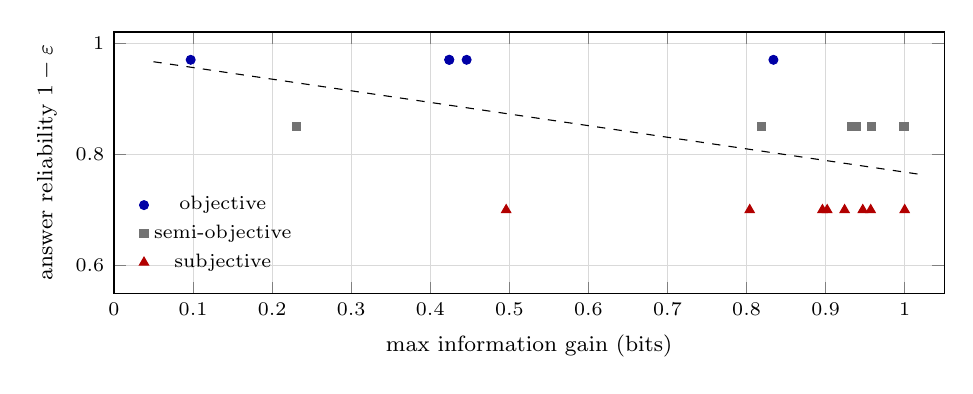
\begin{tikzpicture}
\begin{axis}[
  width=\columnwidth, height=4.9cm,
  xlabel={max information gain (bits)},
  ylabel={answer reliability $1-\varepsilon$},
  xlabel style={font=\footnotesize}, ylabel style={font=\footnotesize},
  tick label style={font=\scriptsize},
  xmin=0, xmax=1.05, ymin=0.55, ymax=1.02,
  grid=both, grid style={line width=0.2pt, draw=black!15},
  legend style={font=\scriptsize, draw=none, fill=none,
                at={(0.02,0.04)}, anchor=south west},
]
\addplot[only marks, mark=*,        mark size=1.6pt, blue!65!black]
  coordinates {(0.097,0.97) (0.446,0.97) (0.424,0.97) (0.834,0.97) (0.424,0.97)};
\addlegendentry{objective}
\addplot[only marks, mark=square*,  mark size=1.5pt, black!55]
  coordinates {(0.958,0.85) (0.939,0.85) (0.999,0.85) (0.819,0.85) (0.933,0.85) (0.231,0.85) (1.000,0.85)};
\addlegendentry{semi-objective}
\addplot[only marks, mark=triangle*,mark size=1.9pt, red!70!black]
  coordinates {(1.000,0.70) (0.902,0.70) (0.957,0.70) (0.924,0.70) (0.804,0.70) (0.896,0.70) (0.947,0.70) (0.496,0.70)};
\addlegendentry{subjective}
\addplot[black, dashed, domain=0.05:1.02, samples=2] {0.977-0.209*x};  % least-squares fit
\end{axis}
\end{tikzpicture}
\caption{Per-attribute maximum information gain (native 2-bin discretisation)
against annotated answer reliability $1-\varepsilon$, with marker shape
indicating tier. Spearman $\rho=-0.438$ ($p=0.054$, $n=20$); the downward
trend is the paper's central empirical claim.}
\label{fig:scatter}
\end{figure}
%----------------------------------------------------------------------

\subsection{Disentangling Selection from Update}

Table~\ref{tab:main} reports top-1 accuracy at the fixed budget for every
method under each noise condition. The comparison of IG+hard against
IG+soft-uniform isolates the update rule with the selection rule held fixed;
the comparison of IG+soft-uniform against RAIG-tiered isolates the selection
rule with the update rule held fixed.

\begin{table*}[t]
\caption{Top-1 accuracy at $T=20$ (\%), mean over $3 \times 300$ paired trials,
with 95\% paired-bootstrap intervals in parentheses.}
\label{tab:main}
\centering
\footnotesize
\begin{tabular}{@{}lcccccc@{}}
\toprule
\textbf{Noise condition} & \textbf{Random+soft} & \textbf{IG+hard} & \textbf{IG+soft-unif.}
& \textbf{IG+soft-obj.} & \textbf{RAIG-tiered} & \textbf{RAIG-oracle} \\
\midrule
Clean ($\lambda=0$) & 0.3 {\tiny (0.0--0.8)} & 96.6 {\tiny (95.3--97.7)} & 96.3 {\tiny (95.1--97.4)} & 0.6 {\tiny (0.1--1.1)} & 41.9 {\tiny (38.8--45.0)} & 96.6 {\tiny (95.3--97.7)} \\
Homogeneous (control) & 0.1 {\tiny (0.0--0.3)} & 15.4 {\tiny (13.1--17.9)} & 23.9 {\tiny (21.2--26.7)} & 0.1 {\tiny (0.0--0.3)} & 9.6 {\tiny (7.7--11.6)} & 23.9 {\tiny (21.2--26.7)} \\
Heterogeneous $\lambda=0.5$ & 0.1 {\tiny (0.0--0.3)} & 14.6 {\tiny (12.3--16.9)} & 20.1 {\tiny (17.6--22.8)} & 0.6 {\tiny (0.1--1.1)} & 17.9 {\tiny (15.4--20.4)} & 26.6 {\tiny (23.7--29.4)} \\
Heterogeneous $\lambda=1.0$ & 0.0 {\tiny (0.0--0.0)} & 2.2 {\tiny (1.3--3.2)} & 2.1 {\tiny (1.2--3.1)} & 0.4 {\tiny (0.1--0.9)} & 7.9 {\tiny (6.2--9.7)} & 7.9 {\tiny (6.2--9.7)} \\
Heterogeneous $\lambda=1.5$ & 0.0 {\tiny (0.0--0.0)} & 0.4 {\tiny (0.1--0.9)} & 0.1 {\tiny (0.0--0.3)} & 0.3 {\tiny (0.0--0.8)} & 3.0 {\tiny (1.9--4.1)} & 2.3 {\tiny (1.3--3.3)} \\
Randomised (control) & 0.0 {\tiny (0.0--0.0)} & 3.4 {\tiny (2.3--4.7)} & 7.3 {\tiny (5.7--9.1)} & 0.2 {\tiny (0.0--0.6)} & 4.3 {\tiny (3.1--5.7)} & 17.4 {\tiny (15.0--19.9)} \\
Adversarial (control) & 0.1 {\tiny (0.0--0.3)} & 8.7 {\tiny (6.8--10.6)} & 14.4 {\tiny (12.2--16.8)} & 0.0 {\tiny (0.0--0.0)} & 3.7 {\tiny (2.4--4.9)} & 23.2 {\tiny (20.6--26.1)} \\
\bottomrule
\end{tabular}
\end{table*}

\subsection{Paired Significance}

Table~\ref{tab:mcnemar} reports exact McNemar tests for the pre-registered
primary comparison and the two comparisons that most threaten the method.

\begin{table}[t]
\caption{Exact McNemar tests, heterogeneous noise at $\lambda=1.0$ ($n=900$
paired trials). $\Delta$ is RAIG-tiered's accuracy minus the comparator's.}
\label{tab:mcnemar}
\centering
\footnotesize
\begin{tabular}{@{}lcccc@{}}
\toprule
\textbf{Comparison} & \textbf{$n_{10}$} & \textbf{$n_{01}$} & \textbf{$\Delta$} & \textbf{$p$} \\
\midrule
RAIG-tiered vs IG+soft-uniform & 65 & 13 & $+5.8\%$ & $1.8\times10^{-9}$ \\
RAIG-tiered vs IG+soft-objective & 69 & 2 & $+7.4\%$ & $2.2\times10^{-18}$ \\
RAIG-tiered vs RAIG-oracle & 0 & 0 & $0.0\%$ & $1.000$ \\
\bottomrule
\end{tabular}
\end{table}

\subsection{Ablations}

Table~\ref{tab:ablation} reports tier granularity and the component ablation;
Fig.~\ref{fig:misspec} reports the misspecification surface. The quantity of
practical interest is the fraction of the oracle--uniform gap recovered by the
three-tier annotation.

\begin{table}[t]
\caption{Ablations at $\lambda=1.0$. $K=2$ merges objective and
semi-objective into one ``reliable'' tier at $\hat\varepsilon=0.09$ (mean of
0.03 and 0.15), keeping subjective at 0.30 -- a partition not specified by the
paper's own $K=3$ scheme and chosen here for this ablation. ``Capacity term
only'' scores questions by $1-\Hb(\hat\varepsilon_{f(q)})$ alone, discarding
split balance $\Hb(p_q\star\hat\varepsilon)$.}
\label{tab:ablation}
\centering
\footnotesize
\begin{tabular}{@{}lcc@{}}
\toprule
\textbf{Variant} & \textbf{Top-1 (\%)} & \textbf{\% of oracle gap} \\
\midrule
$K=1$ (uniform) & 2.1 & 0 \\
$K=2$ & 6.9 & 82.7 \\
$K=3$ (tiered) & 7.9 & 100.0 \\
$K=M$ (oracle) & 7.9 & 100 \\
Capacity term only & 0.0 & $-36.5$ \\
\bottomrule
\end{tabular}
\end{table}

%---------------------------------------------------------------- Fig. 5
\begin{figure}[t]
\centering
\begin{tikzpicture}
\begin{axis}[
  width=\columnwidth, height=4.9cm,
  xlabel={assumed crossover $\hat\varepsilon$},
  ylabel={true crossover $\varepsilon$},
  xlabel style={font=\footnotesize}, ylabel style={font=\footnotesize},
  tick label style={font=\scriptsize},
  xmin=0, xmax=0.4, ymin=0, ymax=0.4,
  grid=both, grid style={line width=0.2pt, draw=black!15},
  colormap/Blues, colorbar, point meta min=0, point meta max=0.80,
  colorbar style={font=\tiny, ylabel={top-1 accuracy}},
]
\addplot[matrix plot*, point meta=explicit,
         mesh/cols=5, mesh/rows=5, mesh/ordering=y varies] table[meta=acc] {
  x     y     acc
  0.02  0.02  0.80
  0.10  0.02  0.79
  0.18  0.02  0.73
  0.26  0.02  0.56
  0.34  0.02  0.49
  0.02  0.10  0.26
  0.10  0.10  0.28
  0.18  0.10  0.21
  0.26  0.10  0.19
  0.34  0.10  0.15
  0.02  0.18  0.06
  0.10  0.18  0.07
  0.18  0.18  0.04
  0.26  0.18  0.06
  0.34  0.18  0.06
  0.02  0.26  0.01
  0.10  0.26  0.01
  0.18  0.26  0.01
  0.26  0.26  0.01
  0.34  0.26  0.02
  0.02  0.34  0.01
  0.10  0.34  0.01
  0.18  0.34  0.00
  0.26  0.34  0.00
  0.34  0.34  0.01
};
\draw[black!45, dashed] (axis cs:0,0) -- (axis cs:0.4,0.4);
\node[font=\tiny, black!60, rotate=45, anchor=south] at (axis cs:0.30,0.30)
  {correct specification};
\end{axis}
\end{tikzpicture}
\caption{Top-1 accuracy (RAIG selector, homogeneous assumed vs. homogeneous
true crossover, $R=100$ trials/cell, $T=20$) as a function of assumed against
true crossover. The diagonal is correct specification. Accuracy is dominated
by the true crossover (rows), falling from 49--80\% at $\varepsilon=0.02$ to
$\le 2\%$ once $\varepsilon\ge0.26$; within a row, accuracy is generally
highest near the diagonal but the effect is small relative to sampling noise
at this grid resolution ($R=100$/cell).}
\label{fig:misspec}
\end{figure}
%----------------------------------------------------------------------

\subsection{Efficiency}

Table~\ref{tab:latency} reports per-turn latency and the Pareto trade-off
between accuracy and query count under threshold stopping.

\begin{table}[t]
\caption{Per-turn selection latency and secondary efficiency metrics,
heterogeneous $\lambda=1.0$, $R=150$ trials, confidence threshold 0.90. At
this noise level the threshold is reached at all for only 0.7\% (IG) / 2.7\%
(RAIG) of trials within $T=20$, so ``Q to threshold'' is effectively censored
at 20 for both and is not a discriminating metric at this noise level.}
\label{tab:latency}
\centering
\footnotesize
\begin{tabular}{@{}lccc@{}}
\toprule
\textbf{Method} & \textbf{ms/turn} & \textbf{Q to threshold} & \textbf{Top-5 (\%)} \\
\midrule
IG+soft-uniform & 68.7 & 20.0 (0.7\% reached) & 10.7 \\
RAIG-tiered & 69.8 & 19.9 (2.7\% reached) & 22.0 \\
\bottomrule
\end{tabular}
\end{table}

%=============================================================================
\section{Discussion}
%=============================================================================

\subsection{Interpretation}

The argument of this paper is deliberately narrow. We do not claim that mutual
information under a stated observation model is a new acquisition function, and
a reviewer who observes that \eqref{eq:raig} follows immediately from
\eqref{eq:channel} is correct. The claim is that the observation model in
attribute-indexed catalogues is heterogeneous in a specific direction that
happens to be adversarial to the naive criterion, that a routine preprocessing
choice amplifies the effect, and that correcting it costs a three-tier
annotation rather than a measurement campaign. Whether the claim survives
contact with data is what Section~VII will decide.

\subsection{Failure Modes}

Three conditions defeat the method, and each is testable. If reliability is
uncorrelated with information gain in a given catalogue, RAIG reduces to
classical IG up to a monotone transformation and yields nothing; the randomised
control measures exactly this. If every attribute is unreliable, no selection
rule helps, because Corollary~\ref{cor:budget} bounds all of them. If the
annotation is inverted---an attribute believed reliable that is not---RAIG will
concentrate queries on it and may underperform the uniform baseline; the
misspecification surface is included to quantify how badly.

A fourth, subtler failure is adversarial or systematically biased users. The
channel model assumes errors are independent of the item, whereas a user who
misunderstands a category will err in the same direction for every item in it.
Such correlated errors accumulate rather than cancel, and neither the update
nor the selector as formulated detects them.

\subsection{Scalability and Generalisation}

Cost is linear in catalogue size and question count, and the compiled
representation makes exhaustive scoring practical at scales where per-turn
recomputation would not be. Nothing in the formulation is specific to music.
Any identification task over an attribute-indexed catalogue with a human oracle
inherits the same structure, and the tiered annotation transfers directly: fault
diagnosis distinguishes measured readings from reported impressions, clinical
triage distinguishes documented history from subjective symptom severity, and
product finders distinguish specifications from preferences. We expect the bias
to be present wherever a catalogue mixes objective identifiers with perceptual
judgements, which is to say almost everywhere, but we have measured it in one
domain and claim it in one domain.

\subsection{Ethical Considerations}

There is an accessibility dimension that we did not anticipate when beginning
this work and that we think is the most interesting implication. A selector
optimising classical information gain preferentially asks the questions
requiring the most domain fluency, because those are the questions whose
answers are least predictable. Users with less domain vocabulary---a casual
listener rather than an enthusiast, a patient rather than a clinician---will
therefore encounter a disproportionate share of questions they cannot answer
well, and will receive systematically worse service from a system that appears
neutral. Reliability-aware selection is, in this reading, a fairness
intervention as much as an efficiency one, and per-user rather than
per-population reliability estimation would sharpen it. We record this as a
direction rather than a result, since we have not measured it.

The interaction data required to estimate reliability is behavioural and
identifying, and per-user estimation would compound that. Population-level
tiers, which is what we advocate, require no per-user data at all.

\subsection{Limitations}
\label{sec:limitations}

The crossover probabilities are assumed rather than measured, which is the
principal limitation and the reason the randomised and adversarial controls are
not optional. The user model is simulated; no human has interacted with the
system, and simulated users are exactly as wrong as the model says they are,
which is the one thing real users never are. Errors are assumed independent
across turns and abstention is not modelled. Attributes are treated as
conditionally independent given the item, which is false for correlated
descriptors such as genre and instrumentation. Finally, results are reported on
a single catalogue.

\subsection{Future Work}

The immediate priority is a human study estimating $\varepsilon_f$ directly and
testing whether the three-tier annotation predicts measured reliability well
enough to justify the deployability claim. Extending the channel to admit
abstention is straightforward analytically: with erasure probability $\delta_f$
the acquisition function becomes
$(1-\delta_f)\left[\Hb(p_q \star \varepsilon_f) - \Hb(\varepsilon_f)\right]$,
and since abstention plausibly correlates with subjectivity in the same
direction as error, the penalty compounds and the bias should be larger than
reported here. Beyond that: online estimation of $\varepsilon_f$ within a
session, correlated error models, per-user reliability profiles, and a
comparison against language-model questioners~\cite{hu2024uot,mazzaccara2024}
on an identical catalogue.

%=============================================================================
\section{Conclusion}
%=============================================================================

Expected information gain is the default criterion for question selection in
interactive identification, and it encodes an assumption that is false whenever
the oracle is human: that answers are observed exactly. We have argued that the
consequence is not merely a loss of precision but a systematic bias, because
the attributes that divide a catalogue most evenly are the vague ones, and
vague attributes are answered worst. Correcting the criterion requires
replacing the split entropy with the mutual information through a per-attribute
binary symmetric channel, which re-ranks candidate questions rather than
rescaling them, admits a capacity-based bound on the query budget, and can be
instantiated from a coarse qualitative annotation instead of measured error
rates. We have also shown that hard candidate elimination is the zero-noise
limit of Bayesian updating rather than a competing design, which removes a
confound present in existing comparative studies of this problem. Whether the
bias is as large as the argument suggests is an empirical question, and the
protocol and controls needed to answer it honestly---including the baseline
that discards unreliable attributes outright---are specified above.

\section*{Acknowledgment}

\textcolor{red}{PENDING.}

\bibliographystyle{IEEEtran}
\bibliography{refs}

\end{document}
